\section{Постановка эксперимента}

Эксперимент NA64 (а также его <<мюонная версия>>, получившая название
NA64mu) использует постановку <<\emph{active beam dump}>> в рамках
которой массивная мишень сама по себе является детектором, а в конкретном
случае NA64 -- гетерогенным (свинец-полиметилметакрилат) электромагнитным
калориметром высокой гранулярности ECAL.

\subsection{Описание установки}

Начатый в 2015-ом году, эксперимент NA64 изначально
был направлен на поиск лёгкого бозона $A'$ получившего в литературе название
<<\emph{тёмный фотон}>> из-за того что гипотетическим механизмом его
образования является редкая конверсия посредством механизма электромагнитного
смешивания, которую можно описать через соответствующую добавку к
электромагнитному слагаемому лагранжиана \acrshort{sm}.

Экспериментальная установка для поиска $A'$ по недостающей энергии
в упрощённом виде изображена на рисунке \ref{fig:setup-schematic-invis}.
Установка состоит из двух калориметров -- электромагнитного
гетерогенного (сэмплирующего) калориметра ECAL, играющего роль активной мишени,
и адронного гетерогенного
калориметра HCAL. Установка снабжена системой мечения частиц, состоящей из
двухплечевого спектрометра на основе газовых микроструктурных трековых
детекторов T1-T4, измеряющих отклонение электронов в поле
магнита~($1.5\text{Тл}$). Триггерная система в простейшем случае
состоит из телескопа быстрых сцинтилляционных счётчиков S1, S2, S3.
Вето-детектор V1 и мюонный счётчик MU1 включаются в триггер в
режиме антисовпадений для исключения гало пучка и подавления мюонного
фона.

\begin{figure}
    \centering
    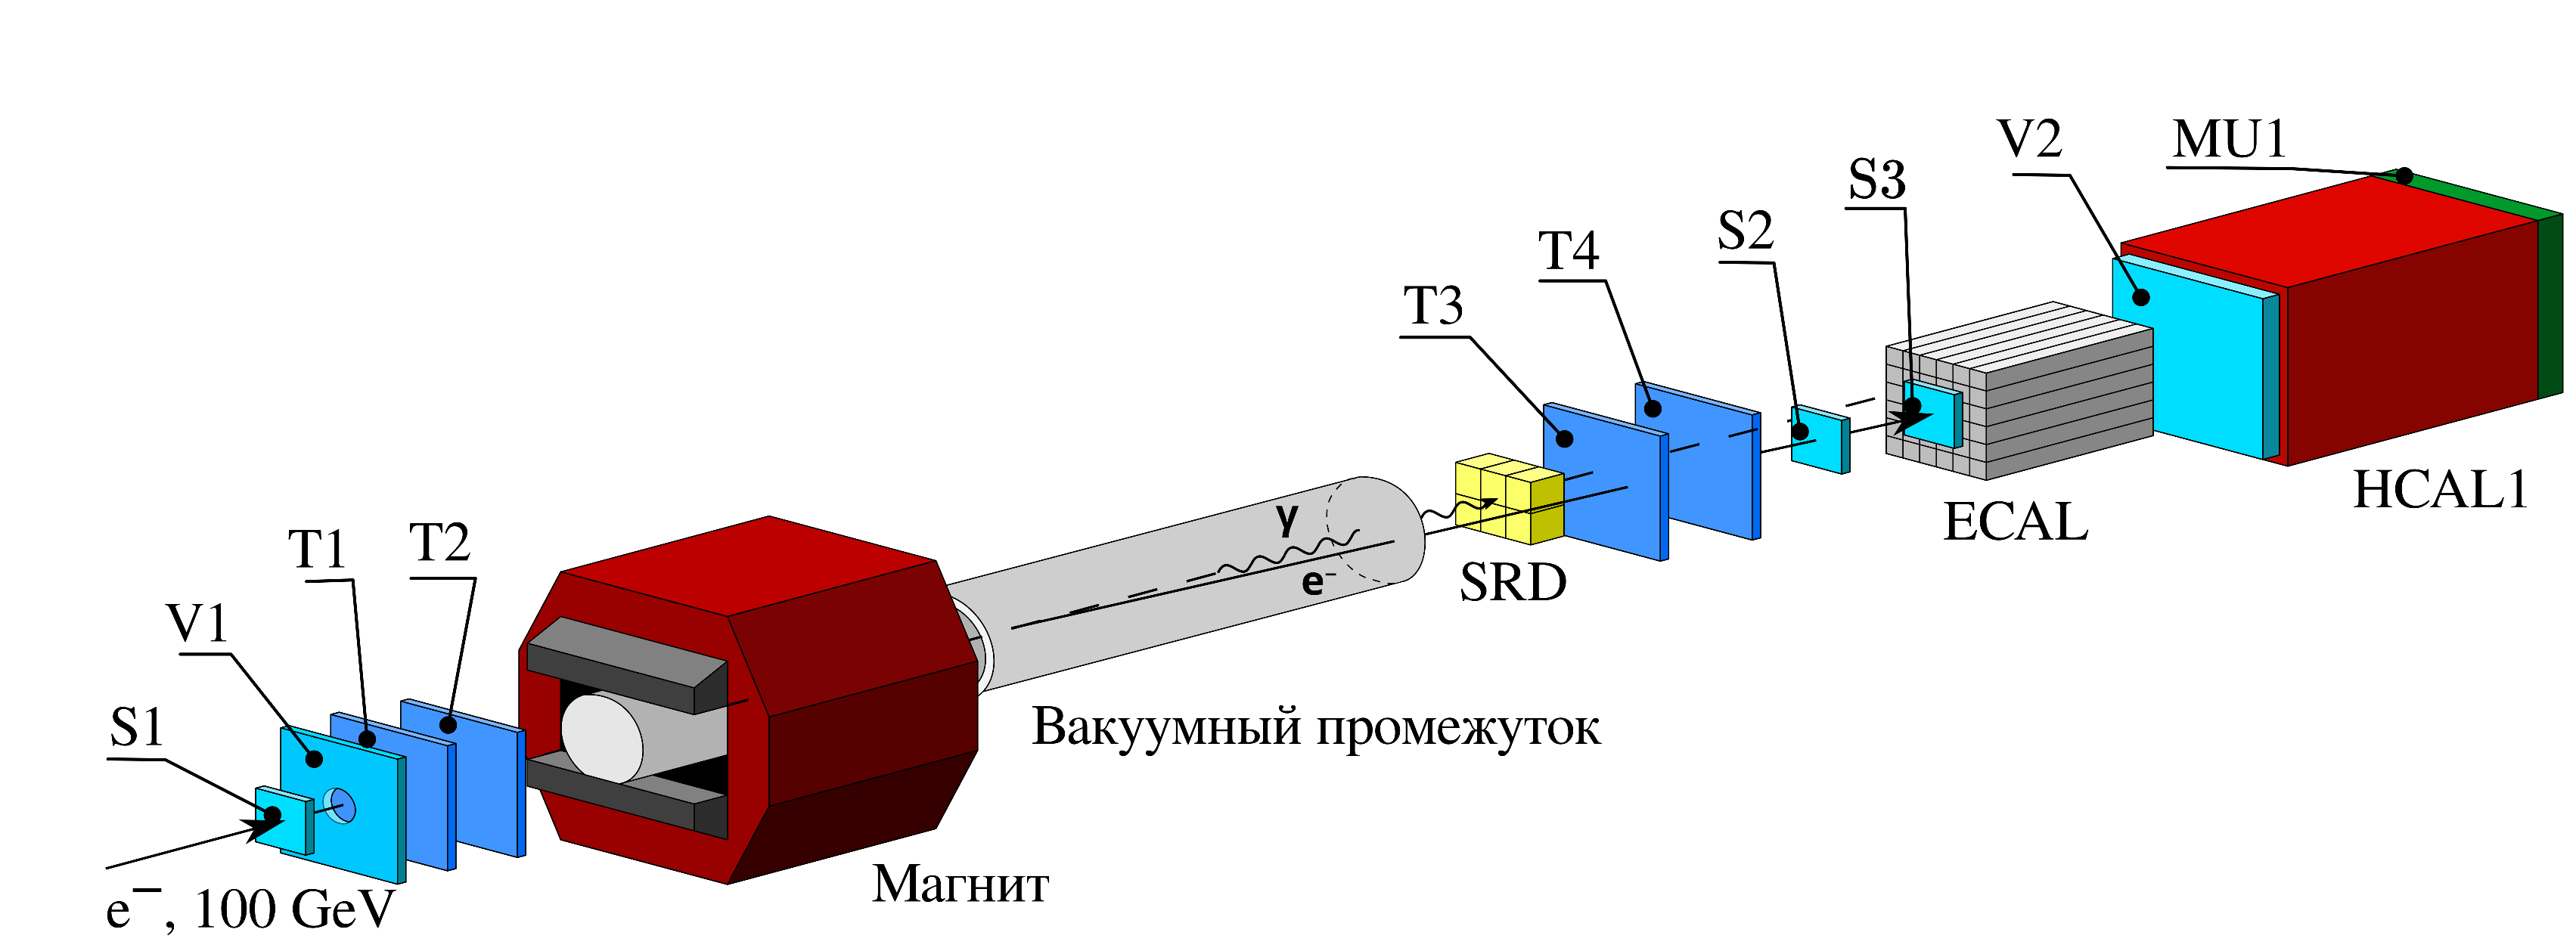
\includegraphics[width=1\linewidth]{images/illustrative/setup-schematic.eps}
    \caption{Размещение детекторов установки NA64 в постановке для обнаружения невидимых частиц}
    \label{fig:setup-schematic-invis}
\end{figure}

Поиск по недостающей энергии заключается в регистрации таких событий,
когда в обоих калориметрах отсутствует существенная часть энергии
инициирующей частицы (несколько десятков ГэВ), что соответствует
образованию высокоэнергетической частицы, способной покинуть
установку без взаимодействия.

Нужно заметить, что ряд процессов \acrshort{sm} в теории способны
реализовать такую сигнатуру: т.н. проникающие (<<пробивные>>,
англ. \emph{punchthrough}) фотоны, нейтральные частицы, мюоны,
альбедо-рассеяние частиц в первых нескольких актах взаимодействия в
мишени и т.д. NA64 оценивает вероятность таких событий менее $10^{-12}$,
что определяет нижний порог чувствительности установки к реакциям такого
типа.

Изображённая на рисунке~\ref{fig:setup-schematic-invis} постановка
может быть существенно модифицирована. Например, с целью подавления фоновых
каналов вместо сцинтилляционного детектора V1 для исключения
адронной компоненты фона в эксперимент в 2018г. были введены сэмплирующие
медные вето-калориметры, трекер дополнен несколькими дополнительными
микропаттерными детекторами и трубчатыми дрейфовыми
детекторами~(\emph{straw}-станциями). Для оценки мюонных фонов
straw-станции низкого разрешения расположены позади адронного калориметра.
В реальности, калориметр HCAL имеет продольную сегментацию, и состоит из
четырёх независимых модулей с поперечной сегментацией $3\times 3$ для
приближённой оценки профиля адронного ливня.

В качестве детектора синхротронного излучения (SRD) в разное время применялись
сегментированные калориметры BGO (из германата висмута), LYSO (ортосиликат
лютеция легированный церием), а так же вольфрам-пластиковые ячейки близкие
по составу к элементам электромагнитного калориметра ECAL.

% TODO: ECAL radiation length
% In order to measure direction of e/m shower and provide good \pi_0 rejection
% (why?) a preshower detector would be required at CMS --- shashlik proposal
% 1993
% TODO: HCAL radiation length

\subsection{Получение пучков и номенклатура данных}

Источником пучка выосокэнергетических ($100~\text{ГэВ}$) электронов в
эксперименте NA64 является ускоритель SPS (\emph{Super Proton
Synchrotron} – протонный суперсинхротрон). Вокруг ускорителя расположены
несколько экспериментальных зон. Эксперимент NA64 проводится в
Северной зоне (\emph{North Area}), включающей в себя два наземных
и один подземный залы, в которых размещены несколько станций вывода
пучка. На этих станциях пучок может выводиться напрямую в зону
эксперимента, либо направляться на мишень-конвертер для генерации пучка
вторичных частиц. Установка NA64 развёрнута на площадке H4,
предоставляющей электронный и адронные пучки. Для
реализации программы NA64mu, оборудование эксперимента перемещается на
площадку M2.

\subsubsection{Конверсия протонов пучка SPS}

В постановке на электронах NA64, пучок протонов с энергией $450~\text{ГэВ}$
интенсивностью $1{,}5 \times 10^{12}$ протонов/на период сбрасывается
на бериллиевую мишень, откуда пучок вторичных частиц передается в
тракт H4, состоящий из набора коллиматоров, отклоняющих и фокусирующих
магнитов, обеспечивающих малый разброс по энергиям и высокую чистоту пучка.

Первичная мишень представляет собой набор из пяти бериллиевых пластин
различной толщины. Толщины пластин составляют 40, 100, 180, 300 и 500~мм.
Пластины установлены в подвижном корпусе окруженном защитой. Соотношение
доли электронов к адронам в конверсионном ливне растет линейно с
увеличением длины мишени. Вторичные адроны образуются в реакциях вида
$p + Z \rightarrow H$ и их доля растёт в линейной пропорции к толщине
мишени $L$, в то время как вторичные электроны в основном являются результатом
распада адронов в реакциях
вида~$p + X \rightarrow \pi^0 \rightarrow \gamma \gamma$, где
аннигиляционные кванты $\gamma$ затем образуют в материале мишени
$e^{+}e^{-}$-пары. Часть из них, пропорциональная $e^{-L}$ поглощается
в веществе мишени. Таким образом, отношение полного выхода электронов и
адронов в конвертере пропорционально $L$ ($L^2 e^{-L}/L e^{-L} = L$),
что позволяет осуществлять эффективную конверсию и сепарацию вторичных
электронов в тракте H4.

Ускорительный комплекс SPS производит вывод пучка периодически --
с периодом в несколько десятков секунд (называемых \emph{суперциклом}),
в течение которых чередуются этапы накопления и сброса пучка.
Сброс пучка длится несколько секунд, остальное время происходит
накопление протонных сгустков в ускорительной ситсеме.

\subsubsection{Номенклатура данных}

К механизму накопления и сброса пучка ускорителя SPS привязана
идентификация событий в данных NA64.

Наиболее общей временной отметкой является отдельный
\emph{экспериментальный сеанс} в течение которого набор
детекторов установки и их взаимное геометрическое расположение
остаются в большой степени неизменными. В течение сеанса
процедуры настройки, калибровки и геометрической юстировки
детекторов производятся заново, обычно в несколько этапов.

С точки зрения накопленных данных, сеансы делятся на набор
пронумерованных подряд \emph{ранов} (англ.~\emph{run}) --
периодов набора статистики с типичной
продолжительностью в один или два часа, в течение которых
экспериментальный зал закрыт и условия набора данных предполагаются
постоянными. Номер рана остаётся уникальным в течение всего
жизненного цикла эксперимента.

Начало и конец рана выдерживаются привязанными к числу актов
сбросов пучка ускорителем. Временной интервал в течение которого
производится квазинепрерывный (банчированный) вывод пучка
называется~\emph{спилл}~(англ. \emph{spill}). Спиллы нумеруются
в ране подряд, и таким образом номер спилла в ране остаётся
уникальным.

Наконец, в пределах одного спилла, нумеруются подряд отдельные
события зарегистрированные триггером.

Таким образом, три числа обозначающие
\begin{itemize}
    \item Номер рана,
    \item Номер спилла,
    \item Номер события в спилле
\end{itemize}
составляют уникальный идентификатор события, который следует
использовать в программной базе эксперимента.

Ожидается, что число ранов NA64 не превысит $10^7$, число
спиллов в ране не превышает $10^3$, а число событий в одном
принципиально ограничено $10^9$. Таким образом, тип данных
для обозначения события потребует мощности в $10^19$ уникальных
значений, что позволяет кодировать идентификатор события
64-разрядным целым числом~($2^{64} \simeq1.85\times10^{19}$),
с сохранением семантики <<ран, спилл, номер события>>.
